\section{Genomförande} % (fold)
\label{sec:genomf_rande}
    \subsection{Fas 1} % (fold)
    \label{sub:steg_1}
        Projektet genomfördes med stöd av den valda metoden. I den första fasen, problemidentifikationsfasen, läggs grunden till projektet. Fas ett strävar efter att skapa en grundläggande förståelse av det problem som projektet avser lösa, samt att möjliggöra fördjupning inom områdets rådande forskningsläge.\bigskip

        För att initiera arbetet behövdes stegen problemidentifikation och problemförståelse genomföras, vilket i detta fall innebar möten med uppdragsgivaren i syfte att få en enhällig uppfattning om vad företaget efterfrågade och att formalisera de praktiska problem till vilka företaget sökte lösning. Vidare var det även i denna fas som introduktionen till projektets rapport utvecklades, som ett ytterligare led i problemidentifieringen och att fastslå vad projektet avsåg utföra. \bigskip

        Den initiala problemanalysen resulterade i att projektet i stort kom att vara uppdelat i två mindre delar, dels den algoritm som kalibrerar panelen och dels en kommunikationslösning mellan panelen och rummet som den levererar ljuset till. \bigskip

        Förutsättningen vid litteraturstudien, gällande kommunikationen mellan taket och byggnadens innandöme, var att den trådlösa kommunikationen skulle ske med standardiserade protokoll. Detta för att underlätta mottagandet av den trådlösa sändningen, i syfte att undvika tidssänken i felsökning då projektet hade en relativt snäv tidsram.\bigskip

        För kalibreringsalgoritmens del bestod problemförståelsesteget av att undersöka vilka typer av datastrukturer som skulle komma att beröras. Det insågs när problemet analyserades att de värden som samlas in kan representeras som en tvådimensionell matris (eng. 'array'), där det finns ett unikt maxvärde och kring detta minskande värden som blir lägre ju längre från maxvärdet de befinner sig, se figur~\ref{fig:array}. \bigskip

        \begin{figure}[hbt]
        \centering
            \begin{subfigure}{0.2\textwidth}
                \pgfplotstabletypeset[color cells={min=5,max=9}, /pgfplots/colormap={yellowred}{rgb255(0cm)=(255,255,105); rgb255(1cm)=(255,10,10)},]
                {
                    5   6   7   6
                    6   7   8   7
                    7   8   9   8
                    6   7   8   7
                }
            \end{subfigure}
            \begin{subfigure}{0.2\textwidth}
                \pgfplotstabletypeset[color cells={min=3,max=9}, /pgfplots/colormap={yellowred}{rgb255(0cm)=(255,255,105); rgb255(1cm)=(255,10,10)},]
                {
                    6   7   8   9
                    5   6   7   8
                    4   5   6   7
                    3   4   5   6
                }
            \end{subfigure}
        \caption{\label{fig:array} Exempel på förväntade fokuspunkter}
        \end{figure}
    % subsection steg_1 (end)

    \subsection{Fas 2} % (fold)
    \label{sub:steg_2}
        Metodens andra fas tar vid när projektet har skapat sig en uppfattning kring vilket problem som ska lösas och vilken forskning som finns inom området. I denna fas läggs förslag till hur problem kan lösas och sedan väljs ett sådant förslag att föras över till nästa fas, fas tre.\bigskip

        Litteraturstudien resulterade i en förståelse av att standarder för trådlös datakommunikation såsom 802.11-standarderna har problem att sända när betongkonstruktioner hindrar utspridningen av radiovågor och speciell apparatur krävs för att klara av att skicka data under sådana förhållanden \cite{11n}. Detta medför att trådlös kommunikation inte är lämplig för företaget, då de på förhand inte kan veta ifall deras kommunikation kommer att fungera på plats hos deras kunder. Inköp av nämnda apparatur är inte aktuellt. \bigskip

        Ett lämpligare medium att kommunicera via är istället de fiberoptiska kablar som redan är dragna, då rummet lyses upp av just dessa kablar. Enligt företaget kommer det finnas mer än en fiberkabel dragen till varje rum, vilket öppnar upp för möjligheten att koppla in apparatur för kommunikation i en fiberkabel, medan den eller de andra kablarna kan fortsätta hämta in ljus till rummet. Med de svårigheter som den trådlösa kommunikationen medförde, i kombination med att ett fungerande alternativt medium redan finns draget, valde projektet att fokusera på det senare. Vid val av kommunikationstillämpning konstaterades att panelens fiberändar har ett reflekterande skydd mot infrarött ljus, enligt \ref{ssub:fiberoptik}, och att ultraviolett ljus inte leds genom panelens yttre glasskiva, vilket leder till att kommunikation över fiberkabeln måste ske med ljus i det synliga spektret. \bigskip

        Det framgick vid datorkörningar att en kalibreringsalgoritm som itererar över hela matrisen för att leta det högsta värdet kommer att vara väldigt ineffektiv. Ett beslut fattades om att utveckla en algoritm som kräver så få steg som möjligt, detta då den praktiska implementationen kommer att innebära fördröjningssteg vid två punkter i körningen, dels när panelen flyttar på sig, och dels när ljuset ska hämtas in från luxmätaren. Algoritmen ska kontinuerligt söka efter ett högre värde tills det maximala värdet är funnet, likt figur~\ref{fig:array}.
    % subsection steg_2 (end)


    \subsection{Fas 3} % (fold)
    \label{sub:steg_3}
        Den tredje fasen i metoden syftar till själva utvecklingen av artefakter, det vill säga att faktiskt framställa någonting som går att använda. Projektet spenderade största delen av projekttiden i denna fas, då varje artefakt utvecklades genom iterationer av de tre delstegen utformning, utveckling och utvärdering. Detta innebar att utveckla en del av artefakten och sedan utvärdera delen för att undersöka hur den beter sig och vad som kan göras bättre.

        \subsubsection{Kommunikationslösning} % (fold)
        \label{ssub:utformning_av_kommunikationslosning}
            Kommunikationsdelen i projektet har genomgått flera iterationer av fas 3 och två huvudlösningar utformades.\bigskip 

            Den första lösningen bestod av två uppsättningar av mikrokontrollerkortet Arduino Uno, för en fullständig specifikation se bilaga~\ref{sub:arduino_spec} \cite{ardu}. En lysdiod kopplades till sändarens gränssnitt som skickar seriell data, vilket då omvandlade den seriella utgångens höga och låga läge till ljus på och ljus av. Till mottagaren kopplades en fotoresistor som ändrar motståndet när den träffas av ljus. När den kopplades in till det seriella gränssnittet skapade resistorn spänningsförändringar som registrerades som högt eller lågt värde av standarden. Vid försök i labbmiljö kunde data sändas med hjälp av lysdioden, driven av 5~V och 20~mA, via fiberkabel om 16 meter och där tolkas från en enskild fiber. För en enkel översikt av kopplingen se figur~\ref{fig:schema}, kopplingsschema finns i bilaga~\ref{sec:kopplingsschema}. Fullständig specifikation finns i bilaga~\ref{sec:specifikationer}.\bigskip

            \begin{figure}
            \centering
                \begin{subfigure}[b]{0.35\textwidth}
                    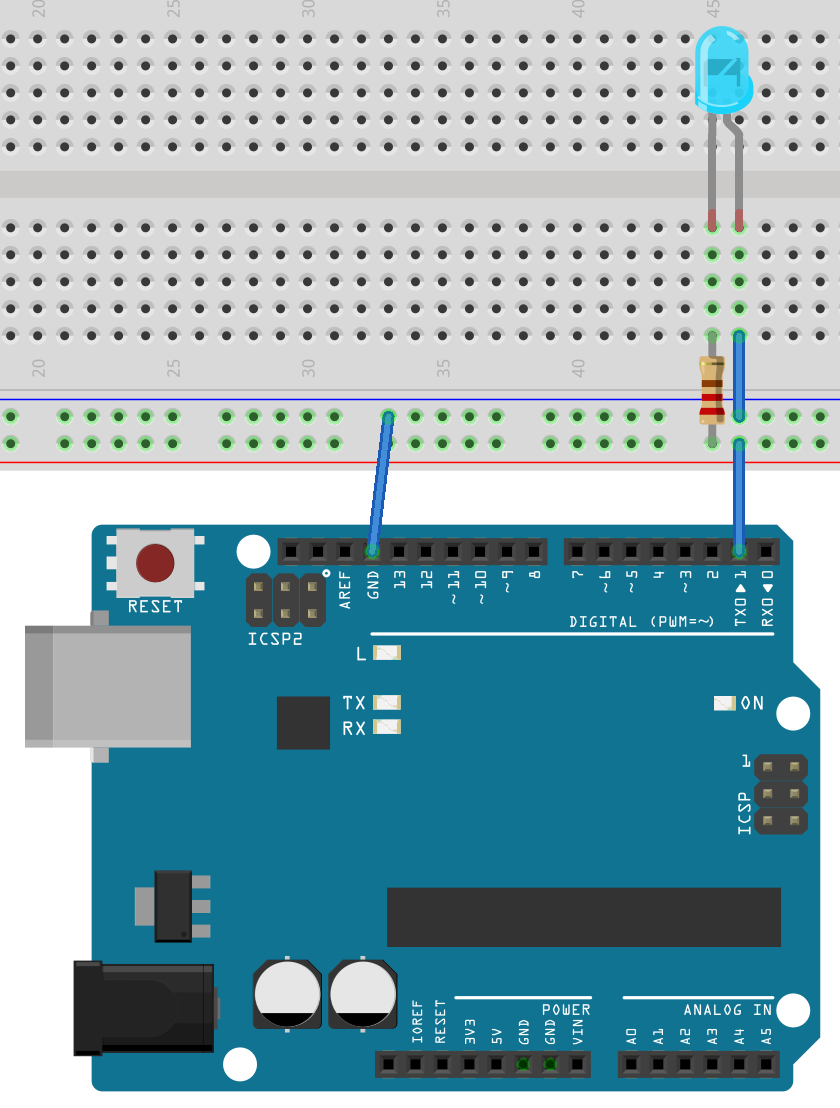
\includegraphics[width=\textwidth]{res/img/led}    
                \end{subfigure}
                \begin{subfigure}[b]{0.35\textwidth}
                    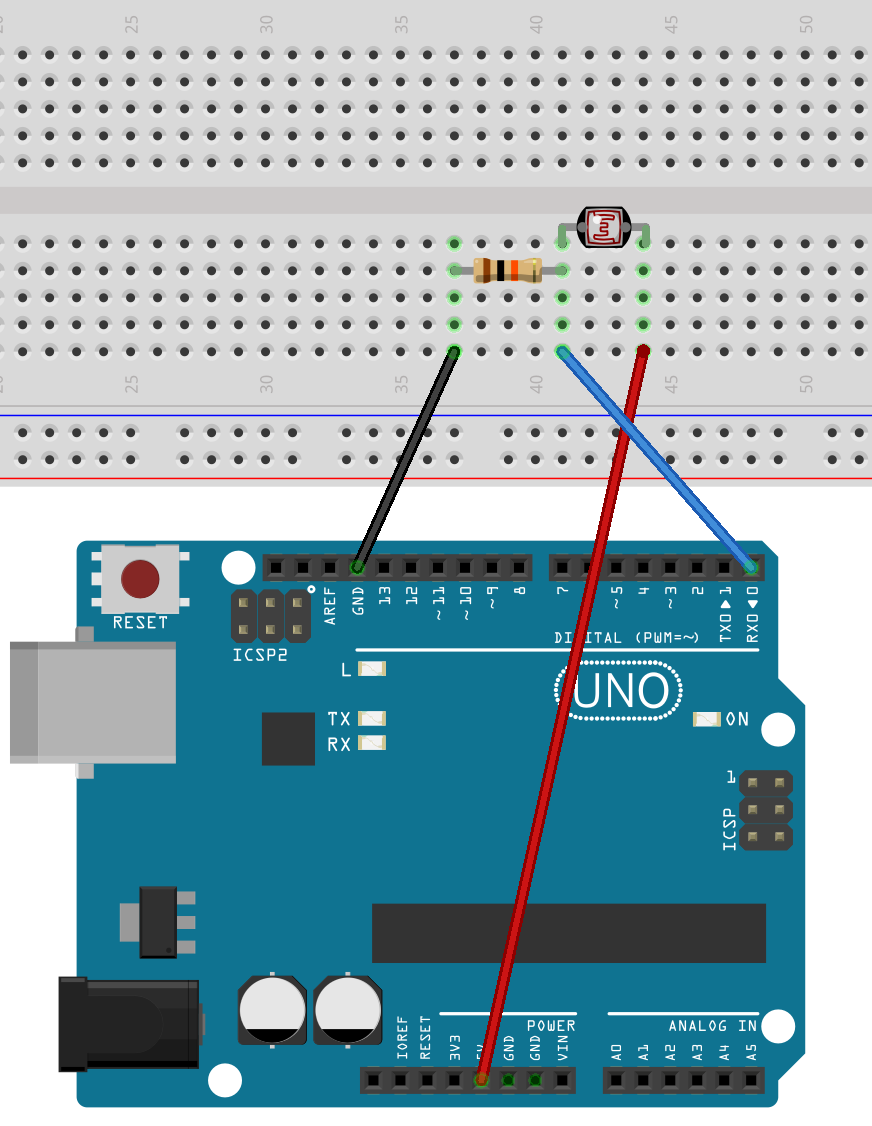
\includegraphics[width=\textwidth]{res/img/resistor}    
                \end{subfigure}
            \caption[Översikt av sändare/mottagare]{Översikt av sändare/mottagare. \\\tiny{Figuren skapad med hjälp av verktyget Fritzing \cite{fritz}}}\label{fig:schema}
            \end{figure}

            För att möjliggöra överföringen användes den i förhållandevis låga överföringshastigheten om 300 baud, vilket gjorde att komponenterna (fotoresistorn och lysdioden) hann ändra sina värden under den tid de förväntades göra det. Komponenterna var inte särskilt utformade för denna uppgift och innehöll vissa fördröjningar vid skifte av tillstånd. \bigskip

            Den data som avsågs skickas i denna kommunikation bestod av ett 16 bitars värde, det vill säga två byte. Med en överföringshastighet om 300 baud ges en teoretisk möjlighet att skicka $\frac{300 \,\textit{baud}}{8 \, bit \cdot 2} = 18,75 \, \text{värden per sekund}$. Den faktiska hastigheten blir något lägre då extra bitar skickas enligt 8N1, men överföringshastigheten var inte att anse som ett hinder i denna implementation. \bigskip
            
            Den andra lösningen använde sig endast av en luxmätare uppe på taket för att inhämta den data som efterfrågades. Genom att koppla samman två fibrer nere i rummet skickas ljuset åter upp till taket och en rundgång i systemet kan skapas. Figur~\ref{fig:loop} visar på linsernas samband med fiberkablarna och genom att koppla ihop kabel 1 med kabel 2 har en återkoppling skapats. Kopplingen kan lämpligen göras med en form av mutter, i fallet att kablarna befinner sig nära varandra, eller med en kopplingskabel. För att minska ljusbortfall rekommenderas lösningen med en mutter när det är möjligt, men om en kopplingskabel behöver nyttjas bör den vara kortast möjligast.\bigskip 

            För att nyttja den här metoden behöver samtliga linser som tillhör en fiberkabel täckas över på panelen för att förhindra att dubbelt intag av solljus transporteras i de båda fiberkablarna, det är även i denna övertäckningsanordning som luxmätaren placeras. Kablarna är anpassade för att hantera den värme som produceras av det ljus som normalt transporteras vid fullt dagsljus men om den dubbla mängden skulle transporteras riskerar fibrerna att smälta på grund av värmebildningen. Lösningen använder sig inte av fiber som bärare av genererad information utan endast det solljus som panelen tar in skickas, vilket minskar både komplexiteten i systemet och risken för störningar.

            \begin{figure}
                 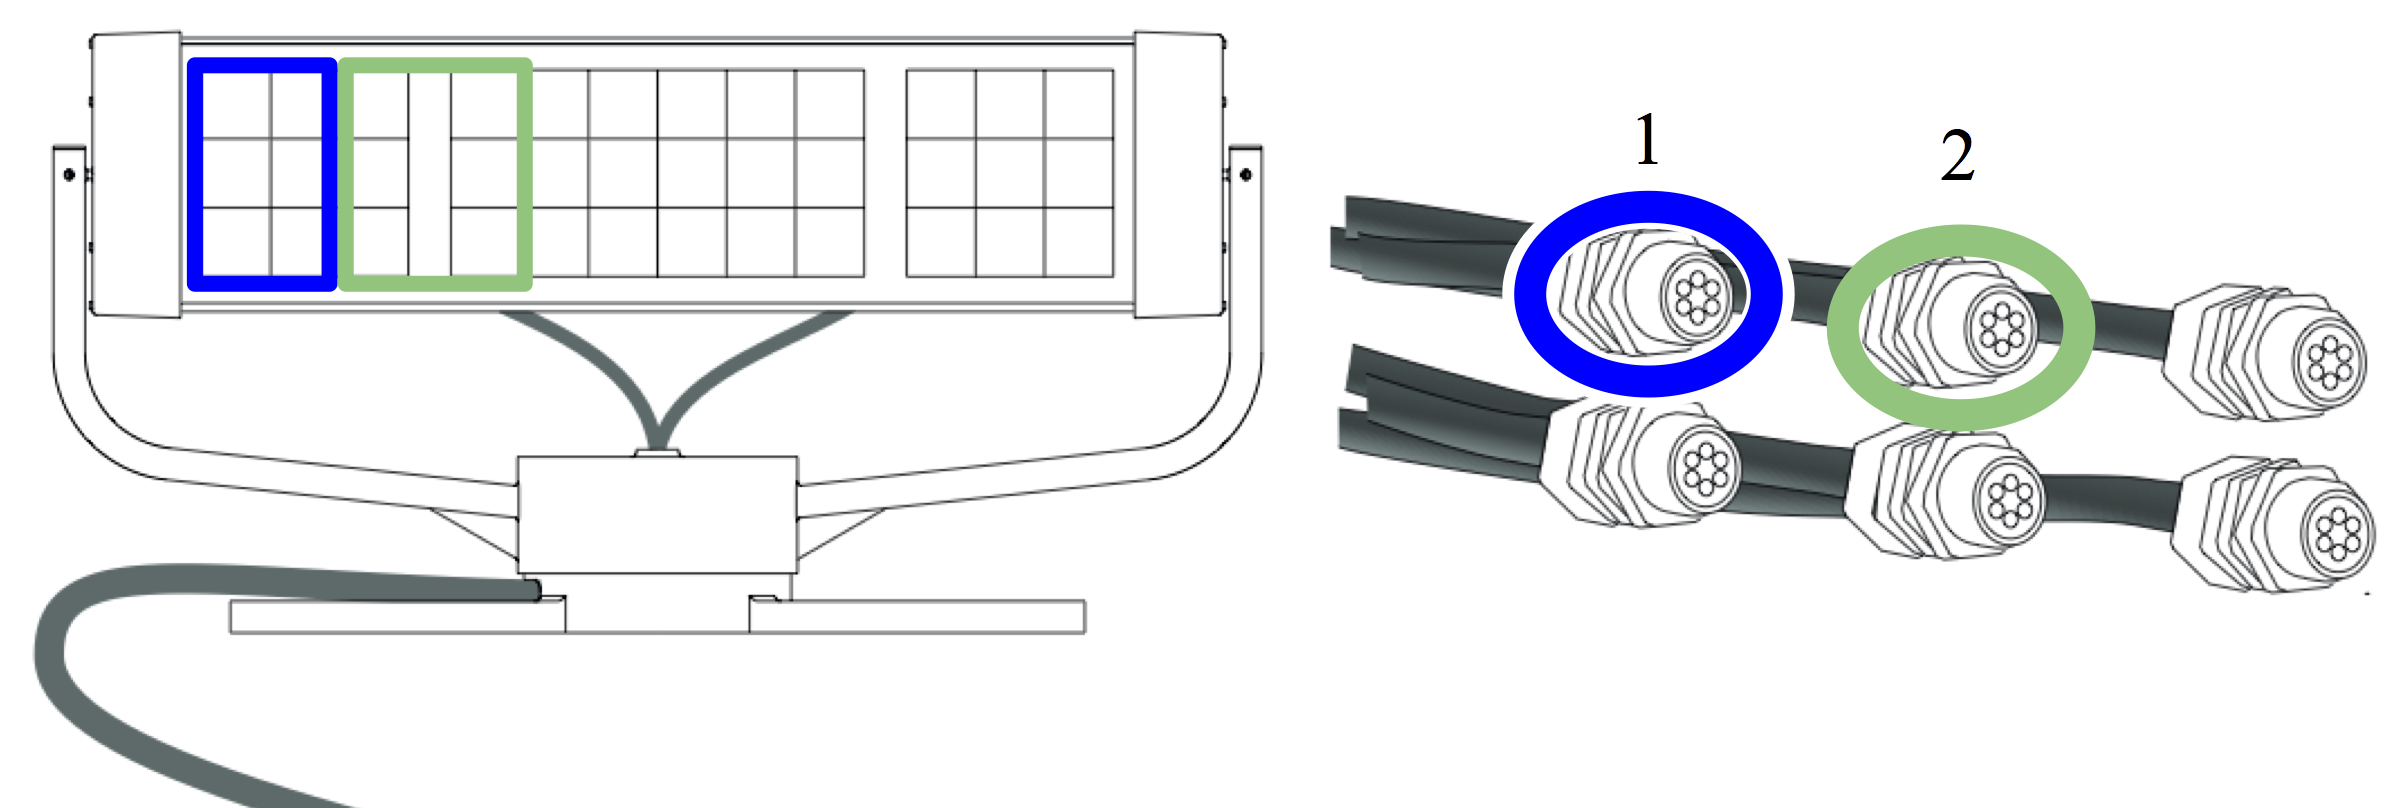
\includegraphics[scale=0.25]{res/img/loop}
            \caption{\label{fig:loop} Översikt av rundgångskoppling}
            \end{figure} 
        % subsubsection utformning_av_kommunikationslosning (end)

        \subsubsection{Avläsning av luxmätare} % (fold)
        \label{ssub:avlasning_av_luxmatare}
            De båda luxmätarna skiljer sig åt med avseende på det gränssnitt som förmedlar data. Mätaren från Adafruit kräver koppling till en mikrokontroller för tolkning av data, medan mätaren från Yoctopuce kopplas direkt till en enhet via USB, vilket underlättar anslutning till en persondator. Även om luxmätarnas gränssnitt skiljer sig åt beter sig de båda snarlikt vid användning. Båda generar ett positivt heltal som representerar uppmätt luxvärde och skickar detta när en metod i respektives bibliotek anropas. Från en programmerares perspektiv är resultatet från och användningen av de båda mätarna i praktiken identisk.\bigskip

            Vid kalibrering av panelen är det av intresse att inhämta så mycket av panelens ljus som möjligt när luxvärdet ska avläsas, samtidigt som bakgrundsljus från andra eventuella ljuskällor undviks, för att skapa mätbara skillnader mellan panelens olika kalibreringssteg. Luxmätaren placeras så nära fiberändan som möjligt för att säkerställa maximalt ljusintag från den panel som ska kalibreras, vilket i praktiken för detta projekt innebär tre till fyra centimeter från fibern. För att hålla mätaren stabil används olika metoder beroende på mätare, där den ena har monterats in i ett metallhölje som skruvas fast på fiberändan, medan den andra vilar i en armatur. Att metoderna skiljer sig åt beror på olika utformning av luxmätarnas mönsterkort och leder till att avlästa värden inte direkt kan jämföras.\bigskip 

            Testning av luxmätarnas inrapporterade värden visade att resultaten från solpanelen fluktuerar, vilket kan bero på orsaker så som att panelen ständigt justerar för att följa solen eller att något som momentant skuggar panelen passerar förbi. Dessa skiftningar i värde är inget som det mänskliga ögat uppfattar men blir synligt i mätningarna. Kompensation för detta kan implementeras med hjälp av mjukvara och projektets lösning beskrivs i avsnitt~\ref{ssub:utveckling_av_applikation}.\bigskip



        % subsubsection avlasning_av_luxmatare (end)

        \subsubsection{Algoritm} % (fold)
        \label{ssub:utveckling_av_algoritm}
            Utformningen av algoritmen skedde genom flera iterationer av steg tre i den valda metoden. I den första iterationen utvecklades en sökalgoritm, algoritm $\mathscr{A}$, som genomförde medurs sökning i åtta riktningar med motsvarande österut som utgångsriktning. När ett större värde påträffats uppdateras nuvarande position och sökningen återupprepas. För jämförelse utvecklades även en variant med fyra sökriktningar, algoritm $\mathscr{B}$. Efterkommande iterationer var samtliga en vidareutveckling av den förra. Den andra iterationen gav algoritmen möjlighet att lagra information om tidigare besökta koordinater, så att dessa ej undersöks vid upprepade tillfällen. Ytterligare förbättringar implementerades i den tredje iterationen, då riktningen på den senaste förflyttningen registreras om ett nytt större värde påträffats. Med hjälp av denna information undersöks först samma riktning som den senast lyckade förflyttningen innan medurs sökning återupptas. Samtliga iterationer innebar märkbara förbättringar vid simulering. Efter tredje iterationen ansågs algoritmen vara funktionsduglig, den använder betydligt färre söksteg än tidigare versioner och hittar effektivt maximipunkten. Ett flödesschema över algoritmen finns i bilaga~\ref{sec:sokalgoritm_flow}.\bigskip

            \begin{figure}
                \pgfplotsset{width=8cm,compat=1.8}
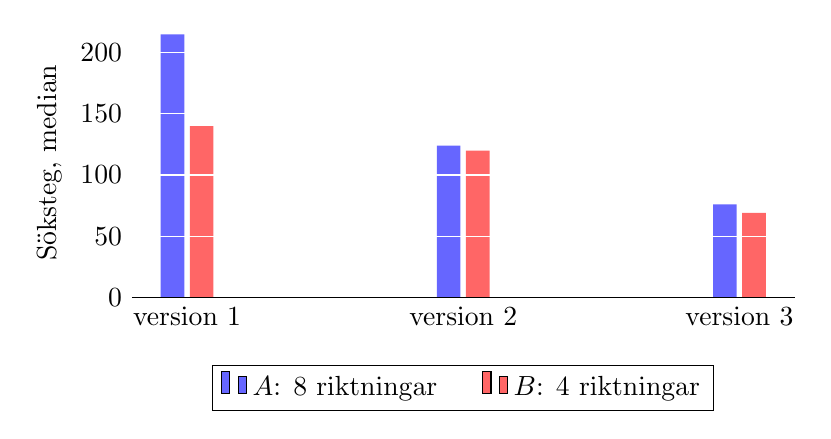
\begin{tikzpicture}
    \centering
    \begin{axis}[
        ybar,
        axis on top,
        % title={Söksteg algoritmer},
        height=5cm, width=10cm,
        bar width=0.3cm,
        ymajorgrids, tick align=inside,
        major grid style={draw=white},
        enlarge y limits={value=.1,upper},
        ymin=0, ymax=200,
        axis x line*=bottom,
        axis y line*=left,
        y axis line style={opacity=0},
        tickwidth=0pt,
        enlarge x limits=true,
        legend style={
            at={(0.5,-0.25)},
            % font=\footnotesize,
            anchor=north,
            legend columns=2,
            /tikz/every even column/.append style={column sep=0.5cm}
        },
        ylabel={Söksteg, median},
        symbolic x coords={version 1, version 2, version 3},
        xtick=data,
        % tick label style={font=\footnotesize},
        ]
        
        %% Median 8 riktningar
        \addplot [draw=none,fill=blue!60] coordinates {
            (version 1,215)
            (version 2,124) 
            (version 3,76)
        };

        %% Median 4 riktningar
        \addplot [draw=none, fill=red!60] coordinates {
            (version 1,140)
            (version 2,120) 
            (version 3,69)
        };
        \legend{$\mathscr{A}$: 8 riktningar,$\mathscr{B}$: 4 riktningar}
    \end{axis}
\end{tikzpicture}
            \caption{\label{fig:algoritm_steg} Jämförelse algoritmernas antal söksteg}
            \end{figure} 

            För att jämföra sökalgoritmerna genomfördes simuleringar som mäter antal steg från utgångspositionen till positionen där maximalt värde påträffas. Simuleringarna använde sig av 10\thinspace000 stycken 100$\times$100-matriser, där varje matris hade en slumpvis genererad utgångsposition och maximalt värde. Algoritmerna genomsökte identiska matriser med samma utgångsposition. Samtliga positioners värden var strängt avtagande med avseende på avståndet till det maximala värdet. För varje iteration av algoritmen undersöktes sökning med både fyra och åtta sökriktningar. Sökning i fyra riktningar visade sig mer effektivt i samtliga fall, enligt figur~\ref{fig:algoritm_steg} och bilaga~\ref{sec:sokalgoritm_sim}. Skillnaderna i antal steg mellan samma algoritm med olika antal sökriktningar vara störst i den första iterationen, med 54~\% fler steg, men de visade sig även i övriga iterationer. I den tredje och slutgiltiga iterationen var skillnaden 10~\% fler steg. Varje iteration av algoritmen minskade det antal steg som behövdes för att finna det största värdet. Största förändringen mellan iterationer skedde mellan iteration två och tre, där antalet steg minskades med 43~\%, se tabell~\ref{tab:algoritm_forbattring}. Minskningen mellan iteration ett och tre var 51~\%. \bigskip

            \begin{table}[b]
                \caption{\label{tab:algoritm_forbattring}Minskning av antal söksteg mellan algoritmversioner}
                \centering
                \begin{threeparttable}
                \begin{tabular}{@{}lcc@{}}
                \toprule
                Från        & \multicolumn{1}{l}{Till version 2} & \multicolumn{1}{l}{Till version 3} \\ \midrule
                Version 1 & 14~\%                                & 51~\%                                \\
                Version 2 & -                                    & 43~\% \\ \bottomrule
                \end{tabular}
                \begin{tablenotes}
                \item Baserat på medianvärden, se bilaga~\ref{sec:sokalgoritm_sim}
            \end{tablenotes}
            \end{threeparttable}
            \end{table}

            Innan algoritmen testades på solpanelen gjordes en undersökning om panelens fokuspunkt överensstämmer med projektets antagande, figur~\ref{fig:array}. 
            En enkel genomsökning av solintaget genomfördes, där panelens justeringsvärden för ljussensorn stegades över ett kvadratiskt fält samtidigt som ljusstyrkan avlästes och fördes in i en tvådimensionell matris.
            Resultatet av denna sökning gav olika bilder beroende på vilken luxmätare som användes. Den ena luxmätarens bild stämde inte överens med antagandet medan bilden från den andra stämde precis, vilket visas i figur~\ref{fig:luxcomp}.
            Hos Parans har tidigare efterforskningar aldrig resulterat i något liknande figur~\ref{fig:ada} och avvikelsen antas bero på luxmätaren Adafruit TSL2591. Att förlita sig till denna mätning skulle ge ett lägre ljusflöde från panelen då dess maximipunkt ligger i utkanten av äkta maximum.
            Projektet beslutade att endast använda den luxmätare som genererade förväntad fokuspunkt, Yoctopuce Yocto-Light-V3.
            Fullständig data från sökningen finns bifogad i bilaga~\ref{sec:heatmap}.

            \begin{figure}[t]
            \centering
                \begin{subfigure}{0.35\textwidth}
                    \setlength{\fboxsep}{0pt}
                    \fbox{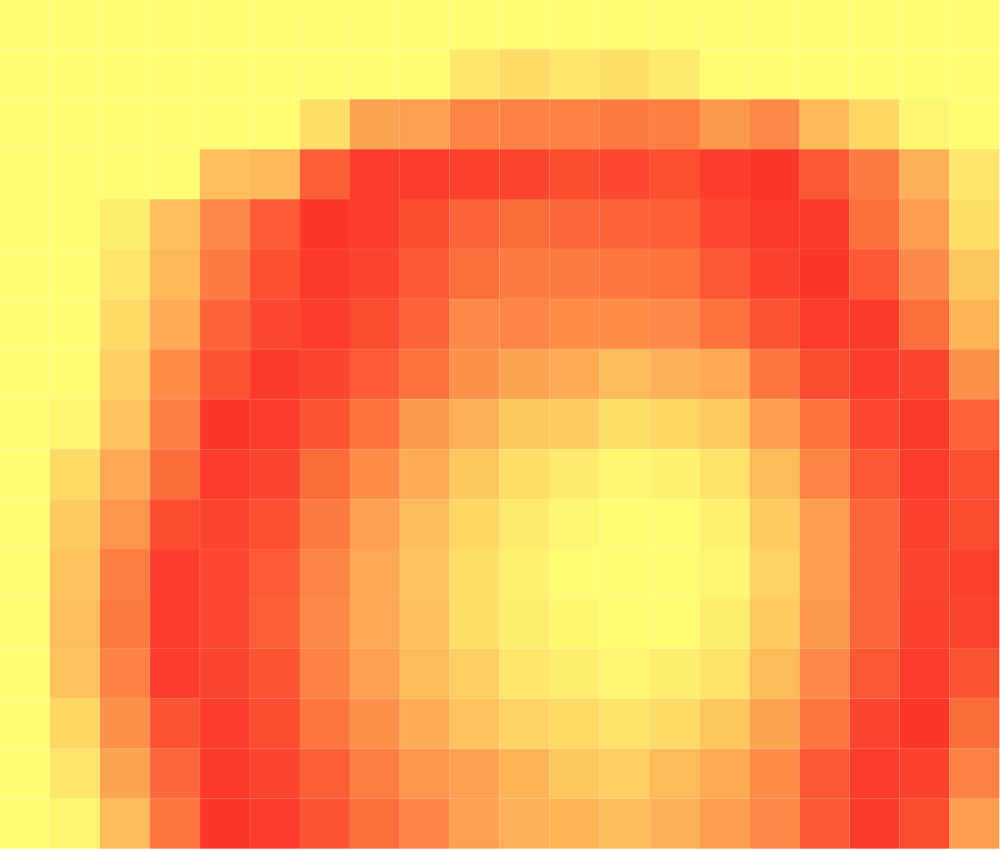
\includegraphics[width=\textwidth]{res/img/new_ada_23}}
                    \caption{\label{fig:ada}Luxmätare från Adafruit}
                \end{subfigure}
                \begin{subfigure}{0.35\textwidth}
                    \setlength{\fboxsep}{0pt}
                    \fbox{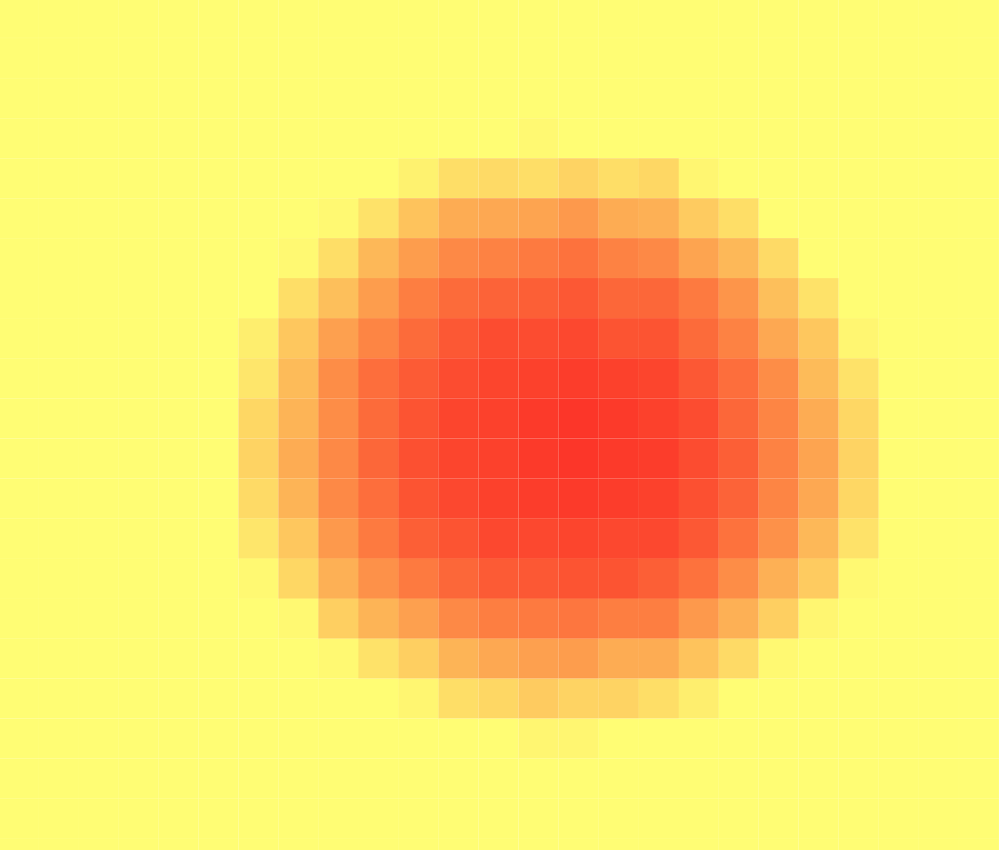
\includegraphics[width=\textwidth]{res/img/old_yocto_23}}
                    \caption{\label{fig:yocto}Luxmätare från Yoctopuce}
                \end{subfigure}
            \caption{\label{fig:luxcomp}Uppmätt ljusstyrka}
            \end{figure}

        % subsubsection utveckling_av_algoritm (end)

        \subsubsection{Applikation} % (fold)
        \label{ssub:utveckling_av_applikation}
            Efter att ha implementerat en algoritm som i simuleringar uppfyllde önskvärd funktion påbörjades utveckling av en applikation där den kan tillämpas. Förutom själva kalibreringsalgoritmen skulle applikationen ha egenskaper som kommunikation med panelen, ett användarvänligt grafiskt gränssnitt och inhämtning av värden från luxmätare. Programmeringsspråket som valdes för utveckling av applikationen var \texttt{Python} och valet hade stöd av flera motiveringar. Den första anledningen till att språket valdes var att företaget har kompetens och erfarenhet att utveckla i detta språk, då den nya panelen SP4 kommer att drivas av en källkod skriven i just \texttt{Python}. Att kompetens och kunskap finns inom företaget medför att applikationen kan underhållas av företaget själv och modifieras vid framtida behov. Vidare har företaget sedan tidigare produkter utvecklade i detta programmeringsspråk, så att utveckla applikationen i samma språk underlättar för en eventuell implementering av mjukvaran i de existerande produkterna. Mer generella fördelar med att utveckla i \texttt{Python} är att språket är plattformsoberoende och är enkelt att utveckla grafiska gränssnitt i. Nackdelar med språket är att det är långsamt i förhållande till andra språk såsom \texttt{C} eller \texttt{Java}. Då applikationen kommer att kommunicera med mekanik, vilket leder till flertalet fördröjningar för rotation av panelen och inhämtning och sändning av information, anser projektet att språkets åverkan på applikationens snabbhet är försumbar \cite{python_speed}. \bigskip

            För att kommunicera med panelen och den Arduino som mottar värden från luxmätaren Adafruit TSL2591 behövdes stöd för seriell kommunikation. Ett bibliotek som möjliggjorde seriell kommunikation med enheter anslutna till en dator var pySerial. Eftersom pySerial har stöd för operativsystem baserade på Windows, Linux och BSD är biblioteket i praktiken plattformsoberoende \cite{pyserial}. 
            Kodbibliotek till luxmätaren Yocto-Light-V3, som anslöts direkt till den dator som kör applikationen, fanns att tillgå från tillverkaren Yoctopuce. \bigskip

            Till det grafiska gränssnittet fanns flera tillgängliga ramverk som var utvecklade för och anpassade till \texttt{Python}. Det som ansågs mest lämpligt för applikation var TkInter, där en anledning var att Parans sedan tidigare hade kringutrustning som använder sig av detta \cite{solarremote}. Hänsyn togs till att för bolaget underlätta både framtida hantering av koden och en eventuell integrering av tidigare produkter med den av projektet utvecklade applikationen. En annan anledning var att ramverket distribueras med standardinstallationer av \texttt{Python} till Windows och Mac OS X \cite{tkinter}. På Linuxsystem behövs TkInter installeras separat och det finns tillgängligt i flera stora Linuxdistributioners pakethanterare. Behovet av extra installationer för ett ramverk kunde minimeras och det grafiska gränssnittet kunde göras plattformsoberoende. \bigskip

            För att underlätta framtida hantering av den producerade koden användes en objektorienterad design av applikationen, där hög kohesion och låg koppling mellan klasserna eftersträvades \cite{java}. Inledningsvis isolerades den framtagna algoritmen i en egen klass, \texttt{Search}. Anslutningarna till panelen och de olika luxmätarna implementerades i separata klasser med specifik kod för att hantera varje enskild enhet. För att hantera de olika anslutningarna skapades klassen \texttt{SerialHandler} som ett mellanliggande gränssnitt till applikationens övriga komponenter. För att kompensera för de fluktuerande värden som beskrevs i avsnitt~\ref{ssub:avlasning_av_luxmatare} hämtar \texttt{SerialHandler} fyra luxvärden från en ansluten mätare och medelvärdet av de två mellersta rapporteras vidare för att få en bättre uppskattning vid kalibreringen. Det grafiska gränssnittet hanteras av klassen \texttt{GUI} och där skapades tryckknappar för att aktivera applikationens funktioner och ett fält för återkoppling och presentation av information. De tre klasserna \texttt{Search}, \texttt{SerialHandler} och \texttt{GUI} fick tillsammans utgöra grundstommen i applikationen och utformades för att vara plattformsoberoende. Genom att sökalgoritmen och det grafiska gränssnittet endast använder sig av det mellanliggande gränssnittet i \texttt{SerialHandler} och ej de underliggande anslutningarna uppnåddes en mer modulär design och ett oberoende av de implementationsspecifika delarna av applikationen. En översikt av klasserna finns i bilaga~\ref{sec:uml_diagram}. \bigskip

            Då applikationen är beroende av anslutning till externa enheter lades funktionalitet till för att underlätta anslutningen. Applikationen kan användas på olika plattformar och olika förfaranden framställdes för olika operativsystem. Stöd för automatisk identifiering av ansluten panel och Arduino implementerades till Mac OS X och Linux. Förutsättningen för detta var att inga fler externa enheter av samma typ är anslutna till den aktuella datorn. För Windowssystem utvecklades en dialogruta som vid applikationsstart frågar användaren efter de aktuella COM-portarna för respektive enhet. Om ingen Arduino är tillkopplad försöker applikationen använda sig av Yocto-Lux-V3. \bigskip

            Det grafiska gränssnittet gavs en enkel design och baserades på det utseende som används i företagets kringutrustning \cite{solarremote}. Nämnda kringutrustning var utformad för att kunna användas med pekskärm och således beaktades detta även här. Fyra knappar i form av ett styrkors lades till för att manuellt ändra panelens justeringsvärden för ljussensorn i x- och y-led. I mitten av styrkorset placerades en knapp för manuell avläsning av den anslutna luxmätaren. Nedanför styrkorset placerades en knapp som startar automatisk kalibrering och en knapp som återställer panelens justeringsvärden till de som var aktuella vid applikationens starttillfälle. Ett fält som kan förmedla aktuell information placerades i applikationens underkant. Det grafiska gränssnittet är avbildat i figur~\ref{fig:app_skiss}.

            \begin{figure}[hb]
                %%% Illustration of the application used for calibration %%%

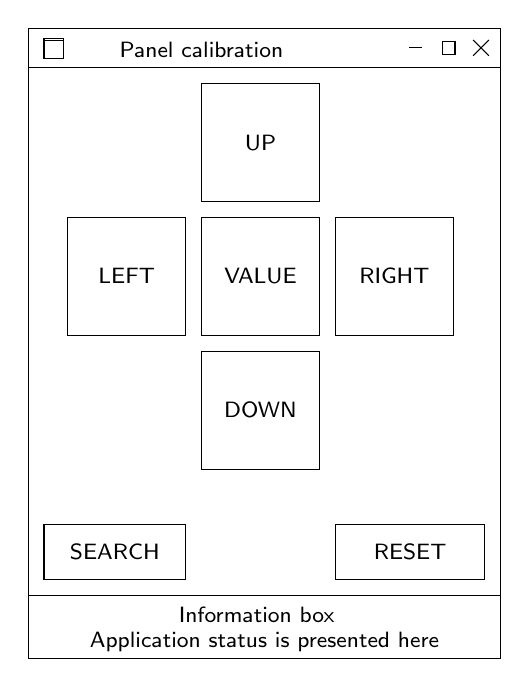
\begin{tikzpicture}[font=\sffamily\footnotesize]
    % Outer rectangle
    \draw (0,0) rectangle (6,8);

    % Top line
    \draw (0,7.5) -- (6,7.5);

    % Bottom line
    \draw (0,0.8) -- (6,0.8);

    % Window functions
    \draw (5.85,7.85) -- (5.65,7.65);           % Close diagonal 1
    \draw (5.85,7.65) -- (5.65,7.85);           % Close diagonal 2
    \draw (5.26,7.67) rectangle (5.42,7.83);    % Maximize (square)
    \draw (4.84,7.75) -- (5.00,7.75);           % Minimize (line)
    \draw (0.2,7.61) rectangle (0.45,7.87);     % Left square
    \draw (0.2,7.84) rectangle (0.45,7.84);     % Line on left square

    % Buttons
    \draw (2.2,7.3) rectangle (3.7,5.8);    % Up
    \draw (0.5,5.6) rectangle (2.0,4.1);    % Left
    \draw (2.2,5.6) rectangle (3.7,4.1);    % Middle
    \draw (3.9,5.6) rectangle (5.4,4.1);    % Right
    \draw (2.2,3.9) rectangle (3.7,2.4);    % Down
    \draw (0.2,1.0) rectangle (2.0,1.7);    % Left corner
    \draw (5.8,1.0) rectangle (3.9,1.7);    % Right corner

    % Text
    \draw (2.2,7.73) node {Panel calibration};
    \draw (2.95,6.55) node {UP};
    \draw (1.25,4.85) node {LEFT};
    \draw (2.95,4.85) node {VALUE};
    \draw (4.65,4.85) node {RIGHT};
    \draw (2.95,3.15) node {DOWN};
    \draw (1.1,1.35) node {SEARCH};
    \draw (4.85,1.35) node {RESET};
    \draw (2.9,0.55) node {Information box};
    \draw (3.0,0.20) node {Application status is presented here};
\end{tikzpicture}

            \caption{\label{fig:app_skiss} Skiss av det grafiska gränssnittet}
            \end{figure}

        % subsubsection utveckling_av_applikation (end)

    % subsection steg_3 (end)

    \subsection{Fas 4} % (fold)
    \label{sub:fas_4}
        Den fjärde fasen i den valda metoden avhandlar inte arbetsgången som sådan, utan visar på att resultatet från den tredje fasen ska analyseras och delges i syfte att sprida kunskapen om vad som har uppnåtts vidare. 
        För detta projekt innebar fas fyra att skriva denna rapport vilket förtydligar och sammanfattar det resultat som har uppnåtts genom de iterationer som genomförts. Vidare hålls en presentation av resultatet inom ramen för den kurs som genomförs, vilket även är en del av metoden.
    % subsection fas_4 (end)
% section genomf_rande (end)